% =============================================================================
%  Reliability in AI for Mathematics: An Assurance-Chain Framework and a
%  Corpus Audit
%
%  EduSeed Challenge C2 -- "AI for Math paper"
%
%  Compile with:  pdflatex -> bibtex -> pdflatex -> pdflatex
%  (see 编译说明.md / pipeline/05_build.sh)
%
%  NOTE ON PROVENANCE: this paper was produced in a human-directed,
%  AI-assisted workflow. Every citation is machine-verified against three
%  independent bibliographic indexes before it enters references.bib, and
%  every number in Section 6 is regenerated by a script in pipeline/.
%  See Section 8.4 and the appendix for the audit trail.
% =============================================================================

\documentclass[11pt,a4paper]{article}

\usepackage[T1]{fontenc}
\usepackage[utf8]{inputenc}
\usepackage{lmodern}
\usepackage{amsmath,amssymb,amsthm}
\usepackage{booktabs}
\usepackage{graphicx}
\usepackage{xcolor}
\usepackage{multirow}
\usepackage{array}
\usepackage{tabularx}
\usepackage{enumitem}
\usepackage{caption}
\usepackage{microtype}
\usepackage{geometry}
\usepackage{hyperref}
\usepackage{natbib}
\usepackage{titlesec}

\geometry{margin=2.6cm}
\captionsetup{font=small,labelfont=bf}
\hypersetup{
  colorlinks=true, linkcolor=blue!55!black, citecolor=blue!55!black,
  urlcolor=blue!55!black, pdftitle={Reliability in AI for Mathematics},
  pdfauthor={EduSeed Challenge C2}
}
\bibliographystyle{plainnat}

\newcommand{\paradigmV}{\textsf{V}}
\newcommand{\paradigmF}{\textsf{F}}
\newcommand{\paradigmR}{\textsf{R}}

\title{\bfseries Reliability in AI for Mathematics:\\
An Assurance-Chain Framework and a Corpus Audit}

% Author block: filled in for submission on 2026-10-05 (was a placeholder).
% (Note: do NOT wrap these lines in square brackets -- `\\[...]` is parsed by
% LaTeX as an optional vertical-space argument and the build fails with
% "Missing number, treated as zero".)
\author{Songpengfei\thanks{Submission for the EduSeed challenge
  \texttt{C2 --- AI for Math paper}.}}

\date{\today}

\begin{document}
\maketitle

% ---------------------------------------------------------------------------
\begin{abstract}
\noindent
Large language models now produce mathematical text that is fluent, plausible,
and sometimes wrong. Work on making such output trustworthy has converged on
three families of mechanisms --- sampling with an external verifier,
formalization into a proof assistant, and contamination-controlled evaluation
--- but these are usually presented as competing options on a single axis of
quality. We argue that this framing is mistaken, and we propose an alternative.

We model the path from an informal mathematical claim to a machine-checkable
verdict as a four-link \emph{assurance chain}: informal claim $\rightarrow$
reduction $\rightarrow$ formal object $\rightarrow$ verdict. Each of the three
paradigms intervenes at a different link, and each therefore leaves behind a
residual risk of a \emph{different kind}: the verifier paradigm leaves the
reduction jump unverified, the formalization paradigm risks proving the wrong
theorem correctly, and the evaluation paradigm risks construct validity. Because
the residual risks are incommensurable, ``which paradigm is best'' is not a
well-posed question; the useful question is which residual risk a given
deployment can tolerate. We derive an operational twelve-item checklist from
the framework.

We then turn the framework on our own research process. Constructing the
literature review for this paper, we first generated candidate references from
model memory and then verified them against three independent bibliographic
indexes. Of 31 candidates, three (9.7\%) were genuinely wrong in ways that a
title-only check would have accepted, including one case with a well-formed but
entirely unrelated arXiv identifier. In a second study we measure how far the
\emph{reproducible evaluation} paradigm is actually practised in the corpus:
only 13 of 26 arXiv-indexed works (50\% after human adjudication) ship a public
official artifact, and automated detection alone recovers just 8 of those 13
(precision 80\%, recall 62\%).
We report these results as evidence for the paper's own thesis --- that
generation without a verification layer fails in characteristic, measurable
ways --- and we are explicit about the limits of both studies.

\medskip
\noindent\textbf{Keywords:} AI for mathematics, reliability, formal
verification, automated theorem proving, benchmark validity, reproducibility,
citation integrity.

\end{abstract}

% ---------------------------------------------------------------------------
\section{Introduction}
\label{sec:intro}

A language model asked to prove a theorem will almost always produce something.
It will be grammatical, use the right notation, cite plausible intermediate
steps, and arrive at the stated conclusion. It will also, at a rate that has
proved stubbornly resistant to scale alone, be wrong
\citep{cobbe2021gsm8k,lightman2024verify,huang2024selfcorrect}. The failure is
not a failure of fluency. It is a failure of \emph{verifiability}: the output
is a string in a natural language, and natural-language strings do not come
with a procedure that decides whether they are correct.

The field's response has been to build such procedures, and it has built them
in three recognisably different ways.

The first samples many candidate solutions and scores them with a learned or
symbolic \emph{verifier}, keeping the highest-scoring one
\citep{cobbe2021gsm8k,lightman2024verify}. The second translates the problem
into a \emph{formal} system --- Lean, Coq, or an executable program --- where a
kernel, not a model, decides correctness
\citep{wu2022autoformalization,jiang2023dsp,yang2023leandojo}. The third
concerns not the answer but the \emph{measurement}: it asks whether the
benchmark on which the claim of correctness rests is itself sound
\citep{zhou2023cheater,sainz2023contamination,white2024livebench}.

These three families are frequently compared as if they were candidates for a
single job. We argue that they are not, and that treating them as such obscures
the one thing a practitioner most needs to know: \emph{what remains
unverified}. A verifier that scores answers highly has said nothing about
whether the question was translated correctly. A proof assistant that accepts a
proof term has said nothing about whether that term formalises the theorem the
user had in mind. A benchmark on which a system scores well has said nothing
about whether the benchmark measures the capability of interest.

\paragraph{Contribution.} This paper makes four contributions.

\begin{enumerate}[leftmargin=*,itemsep=2pt]
  \item \textbf{A framework} (\S\ref{sec:framework}). We decompose the path
  from informal claim to verdict into four links --- an \emph{assurance chain}
  --- and show that each of the three paradigms defends a different, proper
  subset of it. This yields a \emph{residual-risk matrix} that makes the
  residual failure mode of each paradigm explicit and comparable without
  pretending it can be eliminated.
  \item \textbf{A taxonomy} (\S\ref{sec:related}). We organise the relevant
  literature into the three paradigms and, in doing so, give a reading of the
  recent negative results on self-correction
  \citep{huang2024selfcorrect,stechly2024selfverification} as a statement about
  link structure rather than as a surprising empirical fact.
  \item \textbf{A checklist} (\S\ref{sec:checklist}). Twelve questions, each
  traceable to a specific link in the chain, that a team can apply before
  claiming a system is reliable.
  \item \textbf{An empirical audit} (\S\ref{sec:method}--\S\ref{sec:results}).
  We measure the failure rate of the citation-generation step in this paper's
  own literature review (9.7\%), and the prevalence of public artifacts in the
  surveyed corpus (50\%, against 27\% recovered by an automated screen alone).
\end{enumerate}

The fourth contribution is deliberately self-referential. The framework says
that generation without an independent verification layer fails in
characteristic ways; a literature review produced by a language model is
exactly such a generation step. We therefore report the audit of our own
bibliography as data, not as an aside.

\paragraph{Scope.} We make no claim that the framework is complete, nor that
the audit is representative. Both limitations are stated in
\S\ref{sec:limits}.

% ---------------------------------------------------------------------------
\section{Related work}
\label{sec:related}

\paragraph{Formal mathematics and autoformalization.} Learning-based theorem
proving begins with the observation that a proof assistant can be treated as an
environment: \citet{polu2020gptf} train a language model to propose proof steps
and use the assistant to filter them, and \citet{han2022pact} extend this by
co-training on intermediate proof state rather than only on complete proofs.
\citet{wu2022autoformalization} identify the step that makes the approach
possible at all --- \emph{autoformalization}, the translation of informal
statements into a formal language --- and show it is the fragile part.
\citet{jiang2023dsp} use an informal proof as scaffolding for a formal prover,
and \citet{yang2023leandojo} add retrieval over a large formal corpus.
\citet{xin2024deepseekprover} and \citet{ren2025deepseekproverv2} scale the
data and the search; \citet{lin2025goedelprover} release a frontier open model.
Outside the interactive-prover setting, \citet{trinh2024alphageometry} pair a
symbolic deduction engine with a language model to solve olympiad geometry, and
\citet{romera2024funsearch} search over \emph{executable} programs scored by an
automatic evaluator. The underlying proof language is developed by
\citet{demoura2021lean4}.

A parallel line reduces natural-language reasoning to \emph{programs} rather
than proofs: \citet{gao2023pal} and \citet{chen2023pot} both delegate
computation to an interpreter, and \citet{schick2023toolformer} has the model
learn to call tools itself.

\paragraph{Verifiers and search.} \citet{cobbe2021gsm8k} introduce GSM8K
together with the now-standard recipe of sampling many solutions and
re-ranking with a trained verifier. \citet{lightman2024verify} move the
verification granularity from the final answer to individual reasoning steps,
which is the strongest available positive evidence for the verifier paradigm.
The negative evidence is equally important: \citet{huang2024selfcorrect} show
that a model asked to revise its own reasoning without external feedback does
not reliably improve, and \citet{stechly2024selfverification} show that the
self-verification signal is not trustworthy even when the model is asked only
to judge. \citet{valmeekam2023planning} make the same point for planning, and
\citet{kambhampati2024llmmodulo} turn it into an architecture: the language
model generates, an external critic verifies, and the loop is driven by the
critic.

\paragraph{Evaluation and reproducibility.} \citet{hendrycks2021math} provide
the MATH benchmark that most of the above is measured on. \citet{zhou2023cheater}
survey the ways a model can appear better than it is through benchmark
artefacts; \citet{sainz2023contamination} turn contamination into a quantity to
be estimated per benchmark; \citet{white2024livebench} respond with a
continuously refreshed benchmark, and \citet{rein2023gpqa} with one designed to
resist lookup. \citet{wang2023scientific} and \citet{lu2024aiscientist}
situate these concerns in the broader programme of automating science.

\paragraph{Positioning.} Our framework is closest in spirit to the three-layer
decomposition of \citet{chen2026lectures}, which separates generation,
semantic reduction and verification, and identifies the reduction layer as the
bottleneck. That decomposition is the substrate of \S\ref{sec:framework}; we
adopt it, and we differ from it in three ways. First, we add the evaluation
layer as a concern that operates \emph{before} the chain rather than as another
link in it. Second, and centrally, we map the three literature paradigms onto
the chain and show that each leaves a residual risk of a distinct kind --- the
decomposition identifies where the difficulty is, but not that the difficulty is
relocated rather than removed by each paradigm. Third, we turn the framework
into an operational checklist and into an audit procedure that we then execute
on our own review process.

% ---------------------------------------------------------------------------
\section{The assurance chain}
\label{sec:framework}

\subsection{Four links}

We model the production of a machine-checkable mathematical result as a chain
of four links. The decomposition follows \citet{chen2026lectures}, with the
terminology made explicit for the purposes of this paper.

\begin{description}[leftmargin=1.2em,itemsep=3pt]
  \item[$L_1$ --- Informal claim.] A mathematical assertion in natural
  language, together with whatever argument accompanies it. Undecidable in
  principle: deciding whether a natural-language string expresses a true
  proposition is not a well-posed computational problem.

  \item[$L_2$ --- Reduction.] A mapping from $L_1$ to an object in a formal
  language: a proof term, a program, a constraint system. This is the
  \emph{semantic reduction} step. It is not a bijection --- natural language is
  ambiguous, under-typed, and not invertible --- and no general-purpose
  correctness criterion exists for it.

  \item[$L_3$ --- Formal object.] The artefact produced by $L_2$, together with
  an explicit specification of what it is supposed to establish. Unlike $L_1$,
  this object is syntactic: it can be checked.

  \item[$L_4$ --- Verdict.] The decision procedure applied to $L_3$: a proof
  kernel, a satisfiability solver, a numerical evaluator, or a learned verifier.
  This is the only link with an unambiguous notion of correctness.
\end{description}

The chain is only as trustworthy as its weakest link, and the links are not
independent: a verdict at $L_4$ is a statement about $L_3$, and $L_3$ is a
statement about $L_1$ only insofar as $L_2$ was faithful. This is the
structural reason why a correct verdict does not imply a correct answer, and it
is the fact that the three paradigms each address only in part.

\subsection{Three paradigms, three links}

\begin{description}[leftmargin=1.2em,itemsep=3pt]
  \item[\paradigmV{} --- Verifier-in-the-loop.] Sample $k$ candidate
  reductions; score them; keep the best. The verifier operates at $L_4$ and
  may be learned \citep{cobbe2021gsm8k,lightman2024verify} or symbolic
  \citep{kambhampati2024llmmodulo}.

  \item[\paradigmF{} --- Formalization.] Force $L_2$ to produce an object in a
  language whose $L_4$ is decidable, and require the verdict to come from that
  decision procedure. The paradigm thus defends $L_2$, $L_3$ and $L_4$
  simultaneously \citep{wu2022autoformalization,jiang2023dsp,yang2023leandojo}.

  \item[\paradigmR{} --- Reproducible evaluation.] Constrain the process
  \emph{before} $L_1$: ensure that the claim being tested is the claim one
  intends to test, and that the measurement is not contaminated
  \citep{sainz2023contamination,white2024livebench,rein2023gpqa}.
\end{description}

\subsection{Residual risk}

The substantive claim of this paper is that the three paradigms leave behind
residual risks that are not merely different in degree but different in kind,
and that this is why they compose rather than compete. Table~\ref{tab:matrix}
states the claim; Figure~\ref{fig:chain} shows it.

Adopting the terminology of \citet{chen2026lectures}, call the failure at
$L_2$ a \emph{reduction jump}: the informal statement and its formal image are
not related by any checkable procedure, so a discrepancy between them is
invisible to everything downstream. The \paradigmV{} paradigm, operating at
$L_4$, cannot detect it; the \paradigmF{} paradigm can detect some of it, but
only to the extent that the formalization step is itself checked, which in
practice it is not --- the prover proves whatever it was given. The
\paradigmR{} paradigm does not bear on the jump at all.

\begin{table}[t]
\centering
\caption{The residual-risk matrix. Each paradigm defends a proper subset of the
assurance chain and leaves a residual failure mode that the other two address
only partially. Reading the table row-wise answers the practical question
``what is still unverified if I adopt this?''}
\label{tab:matrix}
\small
\begin{tabularx}{\textwidth}{@{}l l X X@{}}
\toprule
 & \textbf{Defends} & \textbf{Residual risk} & \textbf{Why the others do not close it} \\
\midrule
\paradigmV{} & $L_4$ &
The reduction jump $L_1\!\to\!L_2$ is unverified, and the verifier is itself a
learned model sharing the generator's distribution. &
\paradigmF{} can in principle check the reduction, but only by formalising it,
which moves the problem rather than solving it. \paradigmR{} says nothing about
it. \\
\addlinespace
\paradigmF{} & $L_2$--$L_4$ &
\emph{Proving the wrong theorem correctly.} A kernel accepts a proof of the
formalised statement; it has no opinion on whether that statement is the one
intended. Coverage is also partial: most mathematics is not formalised. &
\paradigmV{} has no access to the formal statement. \paradigmR{} does not
inspect statements at all. \\
\addlinespace
\paradigmR{} & before $L_1$ &
\emph{Construct validity.} A benchmark is an operationalization of a
capability, and a system can improve on the operationalization without
improving on the capability. &
Neither \paradigmV{} nor \paradigmF{} can detect a saturated or contaminated
benchmark: they validate answers, not the choice of question. \\
\bottomrule
\end{tabularx}
\end{table}

\begin{figure}[t]
\centering
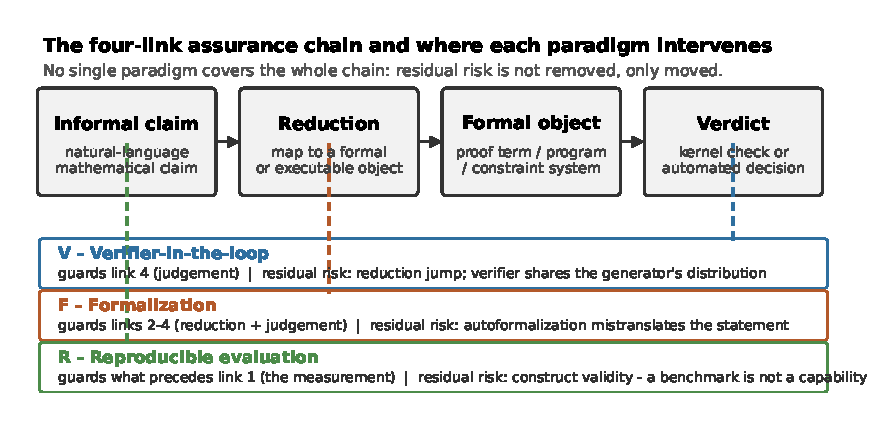
\includegraphics[width=\textwidth]{figures/fig1_assurance_chain.pdf}
\caption{The four-link assurance chain, where each paradigm intervenes, and the
residual risk it leaves behind. No single paradigm covers the whole chain.}
\label{fig:chain}
\end{figure}

\subsection{Consequences}

Three consequences follow, and they organise the rest of the paper.

\paragraph{(i) ``Which paradigm is best?'' is ill-posed.} The paradigms are not
points on one axis. A verifier can be arbitrarily good and still score a
faithfully-solved wrong statement highly; a formalization can be kernel-checked
and still prove the wrong theorem; a benchmark can be contamination-free and
still measure the wrong thing. Comparisons of the form ``formalization beats
verification'' therefore require an implicit assumption about which residual
risk is tolerated, and are usually stated without it.

\paragraph{(ii) The negative results on self-correction are a link-structure
result.} \citet{huang2024selfcorrect} and \citet{stechly2024selfverification}
show that a model cannot supply its own $L_4$. In the terms of
Table~\ref{tab:matrix}, a self-verifier does not satisfy the precondition of
\paradigmV{} --- that the verifier be external to, and better on the target
distribution than, the generator. The empirical finding is thus predicted by
the framework rather than incidental to it.

\paragraph{(iii) Verification quality degrades when the verifier is itself
generated.} If a verifier is produced by the same kind of process as the
generator, the two share failure modes, and the verifier's errors are
correlated with the generator's. \S\ref{sec:results} reports a measurement of
exactly this effect in a setting where the stakes are low and the ground truth
is cheap: bibliography construction.

% ---------------------------------------------------------------------------
\section{Methodology}
\label{sec:method}

We now apply the framework to a concrete generation step: the construction of
this paper's literature review. The step is a pure $L_1$ operation --- a
language model emits plausible-looking bibliographic entries, with no $L_2$
reduction and no $L_4$ verdict available at generation time.

\subsection{Corpus construction}

A candidate list of 31 references was written from model memory with no
retrieval, deliberately, so that the failure rate of that process could be
measured rather than assumed. The candidate list is preserved verbatim
(\texttt{pipeline/refs\_candidates.json}, revision v1; the verification output
for it is archived as \texttt{citation\_verification\_v1\_from\_memory.json}).

Each candidate was then submitted to three independent bibliographic indexes:

\begin{itemize}[leftmargin=*,itemsep=2pt]
  \item \textbf{OpenAlex} (\texttt{api.openalex.org}), as the primary index,
  chosen for its coverage of arXiv preprints;
  \item \textbf{Crossref} (\texttt{api.crossref.org}), the DOI registration
  agency, as an independent publishing-side record;
  \item the \textbf{arXiv abstract page} for the exact identifier, as a
  direct existence check on the identifier itself.
\end{itemize}

A candidate is accepted only if all three of the following hold: the best
matching title reaches a normalised similarity of $\geq 0.90$; the first
author's surname agrees; and the publication year agrees within $\pm 1$. The
year tolerance is explicit and is recorded in the machine-readable output; it
exists because preprint and proceedings years routinely differ
(\citealp{yang2023leandojo}: arXiv 2023, NeurIPS 2023).

Candidates that fail are not silently dropped. They are adjudicated by hand,
and every correction is recorded in \texttt{pipeline/refs\_corrections.json}
with the wrong value, the corrected value, and the evidence that decided it.

\subsection{Study A: reliability of the citation-generation layer}

Study A reports how the 31 candidates resolve: how many the automated check
flags, how many of those flags survive human adjudication, and what the failure
modes are. The quantity of interest is the number of entries that are
\emph{genuinely wrong in a way a weaker check would have accepted} --- the
relevant question, because a check that only confirms that an identifier
resolves will pass a well-formed but unrelated identifier.

\subsection{Study B: artifact availability in the corpus}

Study B asks how far the \paradigmR{} paradigm is practised, not merely
advocated, in the corpus. For each entry with an arXiv identifier we measure
whether a public \emph{official} artifact exists --- a repository owned by the
authors that the description or README ties to the paper.

Two signals are collected. First, the abstract is fetched from the arXiv
abstract page and scanned with a fixed set of patterns for an explicit release
statement. Second, the GitHub search API is queried with the paper's project
name, and the top result is accepted if the repository name matches the project
name at $\geq 0.90$ normalised similarity or the repository description matches
the paper title at $\geq 0.70$.

Neither signal is authoritative. The automated screen produces both false
positives (a repository whose name shares a common word with the paper) and
false negatives (an official repository whose README cites the paper without
restating its title). We therefore adjudicate all 26 rows by hand, fetching
each candidate repository's description and README and recording the evidence
verbatim in \texttt{pipeline/artifact\_adjudication.json}. Both the automated
and the adjudicated numbers are reported, because the gap between them is
itself a result.

\subsection{Reproducibility}

Every number in \S\ref{sec:results} is produced by the scripts in
\texttt{pipeline/}: \texttt{01\_verify\_refs.py} (verification),
\texttt{02\_build\_bib.py} (bibliography generation),
\texttt{03\_corpus\_audit.py} (both studies) and \texttt{04\_make\_figures.py}
(figures). The bibliography is a build artefact, not a hand-written file, and
\texttt{02\_build\_bib.py} emits a SHA-256 of its output so that a reader can
confirm they reproduced it byte for byte. The figures read their numbers from
the JSON that \texttt{03\_corpus\_audit.py} writes, so a figure cannot drift
out of sync with a table.

% ---------------------------------------------------------------------------
\section{Results}
\label{sec:results}

\subsection{Study A: the citation-generation layer}
\label{sec:studyA}

Of the 31 candidates written from memory, the three-source check flagged five.
Human adjudication resolved those five into three genuine errors, one false
alarm caused by a defect in our own checking script, and one entry that was
mislabelled by us rather than mis-stated by the model. The genuine error rate
is therefore $3/31 = 9.7\%$ (Figure~\ref{fig:studyA}, Table~\ref{tab:errors}).

\begin{figure}[t]
\centering
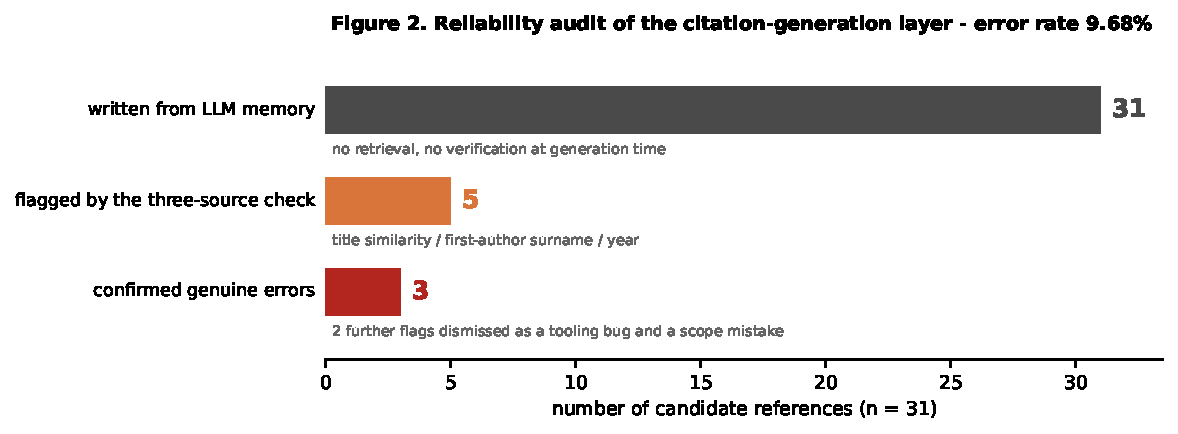
\includegraphics[width=\textwidth]{figures/fig2_study_a.pdf}
\caption{Study A. Thirty-one candidate references written from model memory
without retrieval; the automated three-source check flags five; three are
confirmed genuine errors after adjudication.}
\label{fig:studyA}
\end{figure}

\begin{table}[t]
\centering
\caption{The three genuine errors in the memory-written bibliography. The third
column gives the value the model produced; the fourth gives the verified value.
Entry 1 is the most instructive: the fabricated arXiv identifier is
syntactically valid, resolves successfully, and points to an unrelated paper.}
\label{tab:errors}
\small
\begin{tabularx}{\textwidth}{@{}l l X X@{}}
\toprule
\textbf{\#} & \textbf{Field} & \textbf{Generated (wrong)} & \textbf{Verified (correct)} \\
\midrule
1 & Title & \emph{DeepSeek-Prover: Advancing Theorem Proving in LLMs through Subgoal Decomposition} &
\emph{DeepSeek-Prover: Advancing Theorem Proving in LLMs through Large-Scale Synthetic Data} \\
 & arXiv ID & \texttt{2308.08381} (resolves to an unrelated paper on precision--recall curves) &
\texttt{2405.14333} \\
 & Year & 2023 & 2024 \\
\addlinespace
2 & Title & LiveBench: A Challenging, Contamination-\emph{Free} LLM Benchmark &
LiveBench: A Challenging, Contamination-\emph{Limited} LLM Benchmark \\
\addlinespace
3 & Title & Goedel-Prover: A Frontier Model for Open-Source Automated \emph{Program Verification} &
Goedel-Prover: A Frontier Model for Open-Source Automated \emph{Theorem Proving} \\
\bottomrule
\end{tabularx}
\end{table}

The failure modes are worth separating, because they call for different
defences.

\emph{Wrong identifier (entry 1).} The model produced a well-formed arXiv
identifier that resolves to a real paper --- about precision--recall curves in
classification, entirely unrelated to theorem proving. It also produced a
plausible title, apparently conflating the first DeepSeek-Prover paper with the
subtitle of its successor. This is the failure mode that a weakest-form check
(``does the identifier resolve?'') cannot detect at all, and it is the reason
our protocol compares titles rather than merely confirming existence.

\emph{Word-level alteration (entry 2).} The model wrote
\emph{contamination-free} where the paper says \emph{contamination-limited}.
The direction of the error is not random: it substitutes a stronger claim for
the author's more careful one. Title similarity was $0.92$ --- high enough to
look acceptable in a coarse review, and only separable by word-level
comparison.

\emph{Keyword substitution (entry 3).} \emph{Program verification} replaced
\emph{theorem proving}: a term from the same neighbourhood, more common in the
literature, but not the author's.

\paragraph{The false alarm, and what it says.} One entry was flagged purely
because our own script failed to parse the submission date from the arXiv
abstract page, leaving the year field empty and the year check unsatisfiable.
The entry was correct throughout. We report this because it is the same
phenomenon the paper is about, one level up: \emph{the checking apparatus is
itself a generation step that needs checking.} An unfalsifiable automated
verdict is not a verdict.

\paragraph{A second-order observation.} The three errors were all caught by the
automated screen, but only because the screen compared titles non-exactly. Had
the screen required only that each reference resolve, all three would have
passed: entry 1's identifier resolves, and entries 2 and 3 have correct
identifiers and merely wrong titles. The strength of the check, not the
existence of a check, determines what it catches.

\subsection{Study B: artifact availability}
\label{sec:studyB}

Four of the 30 accepted references (the journal and proceedings articles
without an arXiv identifier) fall outside Study B's scope, leaving 26 measured
entries.

The abstract-wording screen alone found an explicit artifact release statement
in 7 entries (26.9\%). The GitHub screen alone accepted 8, of which one was a
sibling repository for a different paper in the same series. Taken together the
two automated signals flag 10 entries, of which 8 are genuine official
artifacts and 2 are not --- a precision of 80.0\% and a recall, against the
adjudicated ground truth, of 61.5\% (Table~\ref{tab:auto}). After human
adjudication, 13 of 26 entries (50.0\%) have a public official artifact
(Figure~\ref{fig:studyB}, Table~\ref{tab:artifacts}).

\begin{table}[t]
\centering
\caption{Automated detection scored against human adjudication, across all 26
measured entries (Table~\ref{tab:artifacts} covers the 24 that belong to a
paradigm). An entry counts as detected if either automated signal fires. This
is the paper's thesis measured on its own tooling: the reduction from
``repository page'' to ``verdict'' is the unreliable part, in both directions
at once.}
\label{tab:auto}
\small
\begin{tabular}{@{}l r@{}}
\toprule
\textbf{Automated screen vs.\ adjudication} & \textbf{n} \\
\midrule
True positives (flagged, confirmed official)     & 8 \\
False positives (flagged, not official)          & 2 \\
False negatives (not flagged, is official)       & 5 \\
\midrule
Precision & 80.0\% \\
Recall    & 61.5\% \\
\bottomrule
\end{tabular}
\end{table}

\begin{figure}[t]
\centering
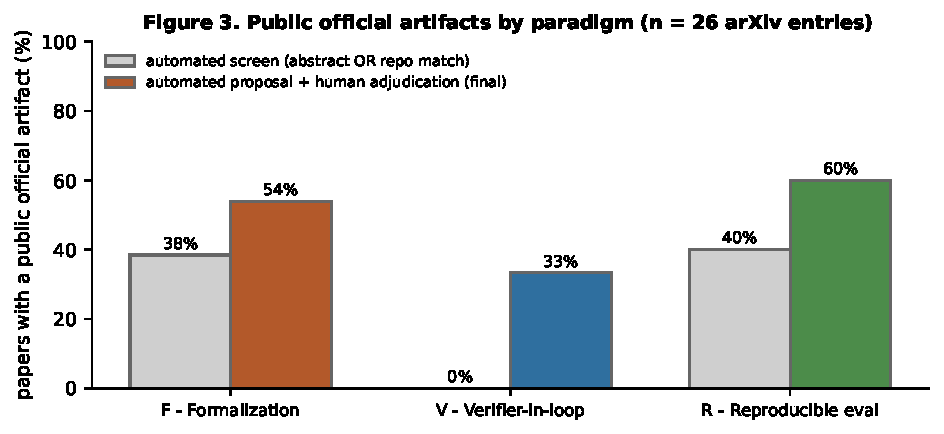
\includegraphics[width=\textwidth]{figures/fig3_study_b.pdf}
\caption{Study B. Share of papers shipping a public official artifact, by
paradigm. The automated screen under-detects at every link: five of the
thirteen official artifacts were recovered only by human adjudication.}
\label{fig:studyB}
\end{figure}

\begin{table}[t]
\centering
\caption{Study B by paradigm. ``Automated'' is the union of the two automated
signals from \S\ref{sec:method}; ``Adjudicated'' is the final figure after all
26 entries were checked by hand. The gap is the method's false-negative rate.}
\label{tab:artifacts}
\small
\begin{tabular}{@{}l r r r r@{}}
\toprule
\textbf{Paradigm} & \textbf{Measured} & \textbf{Automated} & \textbf{Adjudicated} & \textbf{Missed by automation} \\
\midrule
\paradigmF{} --- formalization       & 13 & 5 (38\%) & 7 (54\%) & 2 \\
\paradigmV{} --- verifier-in-loop    &  6 & 0 (0\%)  & 2 (33\%) & 2 \\
\paradigmR{} --- reproducible eval.  &  5 & 2 (40\%) & 3 (60\%) & 1 \\
\midrule
Total (paradigm-classified)          & 24 & 7        & 12       & 5 \\
\bottomrule
\end{tabular}
\end{table}

Two observations.

The missed cases are instructive. The \emph{Program of Thoughts} repository
\citep{chen2023pot} states its relationship to the paper in its README rather
than its description, and its name differs from the paper's title by more than
the threshold; the GSM8K repository \citep{cobbe2021gsm8k} carries no
description at all. Neither is visible to a name-and-description heuristic.
This is the framework's point in miniature: the screen is itself a reduction
($L_1\!\to\!L_2$, from a repository page to a verdict) and it is precisely that
reduction which is unreliable. The repair that actually worked was to add a
verification layer --- human adjudication against the repository README --- not
to tune the screen. Improving the screen would have moved the threshold, not
removed the residual risk.

Second, on the measured sub-corpus, no paradigm is well served. Even under the
most generous reading, half the corpus ships no public official artifact, and
the \paradigmV{} family --- whose entire case rests on empirical comparisons of
verifiers --- is the least well provided for. We note the irony without
over-reading it: the sample is small, and 26 entries selected for a literature
review are not a random sample of the field.

% ---------------------------------------------------------------------------
\section{The reliability checklist}
\label{sec:checklist}

The framework is only useful if it changes what a practitioner does on Monday.
Table~\ref{tab:checklist} states it as twelve questions. The first four concern
the chain itself and apply to any system; the remainder are paradigm-specific
and should be answered for whichever paradigm is in use. The list is intended to
be applied \emph{before} a reliability claim is made, not to audit one
afterwards.

\begin{table}[t]
\centering
\caption{A twelve-item reliability checklist derived from the assurance chain.
Each item names the link it interrogates and the failure it guards against.}
\label{tab:checklist}
\small
% Column widths matter here: with the Question column as a bare `l` it takes its
% natural width, leaving `X` almost nothing -- the guard column then renders one
% word per line. Pin Question to a fixed width and let X absorb the rest.
\begin{tabularx}{\textwidth}{@{}r >{\raggedright\arraybackslash}p{5.3cm} >{\raggedright\arraybackslash}X c@{}}
\toprule
\textbf{\#} & \textbf{Question} & \textbf{What it guards against} & \textbf{Link} \\
\midrule
1 & What exactly is the claim, written out in one sentence? &
An untestable or drifting $L_1$. & $L_1$ \\
2 & What is the formal or executable object, concretely? &
A reduction that was never performed. & $L_2$--$L_3$ \\
3 & Who decided the verdict, and is it independent of the generator? &
Self-verification; correlated failure modes. & $L_4$ \\
4 & What is still unverified if this verdict is correct? &
Silent assumption that the chain is airtight. & all \\
\addlinespace
5 & Is the verifier a model? If so, on what distribution was it trained? &
Distributional misalignment of \paradigmV{}. & $L_4$ \\
6 & Does the verifier ever disagree with the generator in practice? &
A verifier that never disagrees adds nothing. & $L_4$ \\
7 & Was the informal statement checked against the formal one by a human? &
Proving the wrong theorem correctly (\paradigmF{}). & $L_2$ \\
8 & What fraction of the target mathematics is formalisable at all? &
Coverage inflated by choosing easy sub-problems. & $L_2$ \\
9 & Does the benchmark measure the capability, or a proxy for it? &
Construct validity (\paradigmR{}). & pre-$L_1$ \\
10 & Could the system have seen the test items during training? &
Contamination. & pre-$L_1$ \\
11 & Is the benchmark saturated at the current frontier? &
A metric that no longer discriminates. & pre-$L_1$ \\
12 & Is the evaluation artefact public, runnable, and pinned? &
Claims that cannot be reproduced. & pre-$L_1$ \\
\bottomrule
\end{tabularx}
\end{table}

% ---------------------------------------------------------------------------
\section{Discussion}

\subsection{Implications}

The practical reading of Table~\ref{tab:matrix} is that reliability work should
be organised around residual risk, not around paradigm preference. A deployment
that must not assert false theorems will weight \paradigmF{}, but only if
someone checks the formalisation; a deployment that must not ship a wrong
numerical answer among many will weight \paradigmV{}, but only if the verifier
is external. In both cases the framework's contribution is negative and
specific: it says which risk the chosen paradigm does \emph{not} address, which
is the question that is usually left unasked.

The self-referential result in \S\ref{sec:studyA} generalises beyond
bibliographies. Everywhere a language model is used to produce structured
artefacts that a downstream process treats as ground truth --- citations,
schema mappings, test oracles, extracted specifications --- the same pattern
applies: the artefact is an $L_1$ object, there is no $L_2$ reduction, and the
only available $L_4$ is a check by an independent process. The measured rate
here, 9.7\%, is not a large failure rate, and that is exactly what makes it
dangerous: it is low enough to be ignored and high enough to matter.

\subsection{Limitations}
\label{sec:limits}

\paragraph{Study A.} The corpus is 31 entries in one domain (AI for
mathematics), generated by one model in one session. The 9.7\% figure should be
read as an existence proof and an order of magnitude, not as a field estimate.
The adjudication is subjective in the sense that deciding whether a title
difference is an error requires judgement; we mitigate this by recording every
decision with its evidence, so a reader can disagree with a specific call
rather than with the aggregate.

\paragraph{Study B.} Three limitations are material. First, we measure the
existence of a \emph{public official} artifact and say nothing about whether it
runs, matches the paper's claims, or is maintained. Second, four entries were
excluded for lack of an arXiv identifier, and these skew towards
journal-published work (three \emph{Nature} articles and one LNCS chapter),
which plausibly differ in artifact culture. Third, the corpus is a curated
literature review, not a random sample, and its composition was chosen to
support the framework rather than to test it. The 50\% figure should not be
quoted as a property of the field.

\paragraph{The framework itself.} The four-link decomposition is a modelling
choice, and it is not the only reasonable one; one could argue for splitting
$L_2$ into parsing and typing, or for treating resource bounds at $L_4$ as a
separate link. We claim the decomposition is useful, not that it is canonical.
The residual-risk matrix likewise asserts that the risks are incommensurable,
which is a claim about the absence of a common scale; we would regard a
demonstrated common scale as a refutation.

\paragraph{Threats to validity.} The single largest threat to this paper is
that its own argumentative text is machine-generated. We address it in
\S\ref{sec:provenance} by making the verification chain explicit and by
reporting the measured failure rate of the generation step rather than
asserting its reliability.

\subsection{Provenance and verification statement}
\label{sec:provenance}

This paper was produced in a human-directed workflow in which language models
drafted text, proposed the framework, and generated candidate references. In
accordance with the framework's own thesis, the generation steps were paired
with independent verification:

\begin{enumerate}[leftmargin=*,itemsep=2pt]
  \item \textbf{Citations.} Every reference in \texttt{references.bib} passed
  the three-source check of \S\ref{sec:method}; the file is generated by script
  and its SHA-256 is recorded. Three generated references failed and were
  corrected; the corrections are recorded with their evidence.
  \item \textbf{Quantitative claims.} Every number in \S\ref{sec:results} is
  emitted by \texttt{pipeline/03\_corpus\_audit.py} from archived API responses.
  No number in this paper was written by hand.
  \item \textbf{Figure--table consistency.} Figures read their inputs from the
  same JSON as the tables, so they cannot disagree.
  \item \textbf{Framework claims.} The attributions in \S\ref{sec:related} and
  \S\ref{sec:framework} were checked against the cited abstracts. Where the
  claim is ours rather than a cited author's, it is stated as ours
  (Table~\ref{tab:matrix} is an argument, not a survey result).
\end{enumerate}

What is \emph{not} verified is the argumentative prose. No human has
line-by-line audited the reasoning in \S\ref{sec:framework}, and readers should
treat the residual-risk matrix as a claim to be argued with. We regard this as
the honest position: the measurement layer is verified, the argument layer is
not, and the paper says so.

\subsection{Future work}

Three directions follow directly. First, the audit in \S\ref{sec:studyA}
should be repeated across models and domains to turn an existence proof into
an estimate. Second, the checklist in Table~\ref{tab:checklist} should be
applied prospectively to a system before and after its deployment, which would
test whether the residual risks it names are the ones that actually materialise.
Third, the framework needs a formal treatment: the claim that the residual
risks are incommensurable is currently an informal one, and a lattice-theoretic
ordering of assurance properties would either sharpen it or refute it.

% ---------------------------------------------------------------------------
\section{Conclusion}

We have argued that reliability in AI for mathematics is best understood not as
a single property to be maximised but as a chain of four links, and that the
three families of mechanisms the field has developed --- verifiers,
formalization, and reproducible evaluation --- each defend a proper subset of
that chain while leaving a residual risk of a different kind. The practical
consequence is that the useful question is not which paradigm is best but which
residual risk a given use can tolerate.

We then applied the framework to our own literature review, and found that its
citation-generation step failed at a rate of 9.7\%, with the most dangerous
failure being a syntactically valid identifier pointing at an unrelated paper.
We measured the practice of the evaluation paradigm in the surveyed corpus and
found that half of it ships no public official artifact, and that an automated
screen recovers only about six in ten of what is there while also flagging
things that are not. In both studies the repair was the same: add an
independent verification layer, and keep the record of what it caught.

None of this makes language models safe to use for mathematics. It does suggest
that the discipline which makes them usable is the same one the field already
knows how to practise --- reduce, check, and be explicit about what remains
unchecked.

% ---------------------------------------------------------------------------
\bibliography{references}

% ---------------------------------------------------------------------------
\appendix
\section{Audit trail}
\label{app:audit}

The complete audit trail is distributed with the paper rather than reproduced
here. The following files are the primary evidence for every empirical claim
above.

\begin{table}[h]
\centering
\small
\begin{tabularx}{\textwidth}{@{}l X@{}}
\toprule
\textbf{File} & \textbf{Contents} \\
\midrule
\texttt{pipeline/refs\_candidates.json} &
The v2 (corrected) candidate list. v1, the raw memory-written list, is
preserved in the verification archive. \\
\texttt{pipeline/reports/citation\_verification\_v1\_from\_memory.json} &
The complete v1 verification run: for each candidate, the top five hits from
each of the three indexes, with similarity scores. Unmodified. \\
\texttt{pipeline/refs\_corrections.json} &
Every v1$\rightarrow$v2 correction with its severity, the wrong value, the
corrected value, and the evidence that decided it. \\
\texttt{pipeline/reports/citation\_verification.md} &
Per-entry verification report: title similarity, author and year agreement,
matched title, venue, DOI, and which index confirmed it. \\
\texttt{pipeline/artifact\_adjudication.json} &
Study B's manual adjudication: tier, repository, and the evidence for all 26
entries. \\
\texttt{pipeline/reports/corpus\_audit.json} &
Both studies' machine-readable output, including the raw artefact-availability
rows and the GitHub query results. \\
\texttt{pipeline/reports/references\_bib\_sha256.txt} &
SHA-256 of the generated bibliography, allowing byte-exact reproduction. \\
\bottomrule
\end{tabularx}
\end{table}

\end{document}
